% !TeX root = ../CommonRoad_Format.tex


\section{CommonRoad Map}

\subsection{Location of Scenarios} \label{subsec:location}
The location element consists of (1) a GeoName-ID\footnote{\href{https://www.geonames.org/}{geonames.org}}, (2) a GPS latitude coordinate, (3) a GPS longitude coordinate, (4) an optional geometrical transformation introduced in the following subsection.
If the GeoName-ID and the GPS coordinates are unknown, e.g., in artificial road networks, the GeoName-ID is set to -999 and the values of the coordinates are set to 999.

\subsection{GeoTransformation Element}
\label{para:geo_reference}

To specify the geometrical transformation which were performed while creating the lanelets, one can add a \texttt{geoTransformation} element. This may contain two children:

\begin{enumerate}
	\item The optional \texttt{geoReference} element contains a \emph{proj-strings}\footnote{\href{https://proj.org/usage/quickstart.html}{proj.org}} describing a coordinate transformation from geodetic coordinates to the projected (Cartesian) coordinates. This projection can then be used to transform the Cartesian coordinates back to geodetic coordinates used by OSM (cf. Sec.~\ref{sec:OSM}).
	\item The \texttt{additionalTransformation} element (see Fig.~\ref{fig:additionalTransformation}) describes geometrical operations which were performed (after the geoReference) to transform the Cartesian coordinates. The execution order of the transformations is according to the order of the following list:
	\begin{itemize}
		\item \texttt{xTranslation} Translating x-coordinates of all points by this value.
		\item \texttt{yTranslation} Translating y-coordinates of all points by this value.
		\item \texttt{zRotation} Rotating all points by this value around the origin, with respect to a right-handed coordinate system.
		\item \texttt{scaling} Multiplying all x- and y-coordinates by this value.
	\end{itemize}
\end{enumerate}
\begin{figure}[!htpb]
	\centering
	\begin{minipage}{7.5cm}
		\small
		\dirtree{%
			.1 /.
			.2 [0..1] additionalTransformation.
			.3 [1] xTranslation.
			.3 [1] yTranslation.
			.3 [1] zRotation.
			.3 [1] scaling.
		}
		\caption{Element \textit{additionalTransformation}}
		\label{fig:additionalTransformation}
	\end{minipage}
\end{figure}

\subsection{Lanelets} \label{subsec:lanelets}
We use {\it lanelets} \cite{Bender2014} as drivable road segments to represent the road network.
Fig.~\ref{fig:structure} shows the specification of a \textit{lanelet} element.
It is defined by its {\it left} and {\it right boundary}, where each boundary is represented by an array of points (a polyline), as shown in Fig.~\ref{lanelet1}.
Optionally, line markings (solid, dashed, broad solid, broad dashed, no line marking, unknown, where unknown is the default line marking) can be included to model the boundary more precisely.
We have chosen lanelets since they are as expressible as other formats, such as e.g. OpenDRIVE\footnote{\href{http://www.opendrive.org}{opendrive.org}}, yet have a lightweight and extensible representation.
Our converter from OpenDRIVE to Lanelets is available on our website.

A lanelet consists of the following elements:
%\begin{itemize}
%3 [1] leftBound.
%.4 [2..N] point.
%.4 [0..1] lineMarking.
%.3 [1] rightBound.
%.4 [2..N] point.
%.4 [0..1] lineMarking.
%.3 [0..N] predecessor (\textrm{ref to} lanelet).
%.3 [0..N] successor (\textrm{ref to} lanelet).
%.3 [0..1] adjacentLeft (\textrm{ref to} lanelet, \textrm{drivingDir}=same/opposite).
%.3 [0..1] adjacentRight (\textrm{ref to} lanelet, \textrm{drivingDir}=same/opposite).
%.3 [0..1] stopLine.
%.3 [1..N] laneletType: highway/urban/busStop/.../crosswalk.
%.3 [0..N] userOneWay: vehicle/car/truck/bicycle/.../pedestrian.
%.3 [0..N] userBidirectional: vehicle/car/truck/bicycle/.../pedestrian.
%.3 [0..N] trafficSignRef (\textrm{ref to} trafficSign).
%.3 [0..N] trafficLightRef (\textrm{ref to} trafficLight).
%\end{itemize}


\begin{figure}[!htpb]
	\centering
	\footnotesize
	\psfrag{a}[l][c]{lanelet (road)}
	\psfrag{b}[l][c]{lanelet (rail)}
	\psfrag{c}[l][c]{road vehicle}
	\psfrag{d}[l][c]{tram}
	\psfrag{e}[l][c]{\shortstack[l]{driving \\[-0.05cm] direction}}
	\psfrag{f}[l][c]{ego vehicle}
	\psfrag{g}[r][c]{right boundary}
	\psfrag{h}[r][c]{left boundary}
	\psfrag{i}[l][c]{\shortstack{lanelets of \\ equal length}}
	\psfrag{j}[l][c]{\shortstack{point of \\ polyline}}
	\includegraphics[width=0.9\columnwidth]{figures/stachus_uniColor_d.eps}
	\caption{Lanelets of a complex intersection in the city center of Munich. Besides roads, also tram rails are modeled by lanelets.}
	\label{lanelet1}
\end{figure}

In order to represent the graph of the road network, the elements \textit{predecessor}, \textit{successor}, \textit{adjacentLeft}, and \textit{adjacentRight} are used, which are omitted if they are empty (see Fig.~\ref{fig:structure}).
Since these elements only contain objects which are already existing, we refrain from copying their data but introduce references to the neighboring lanelets by an attribute referring to their unique ID.
The elements \textit{predecessor} and \textit{successor} can be used multiple times to represent multiple longitudinally adjacent lanelets, e.g., for a road fork.
In contrast, a lanelet can have at the most one \textit{adjacentLeft} and one \textit{adjacentRight} neighbor and thus at the most one element of this type.
The additional attribute \textit{drivingDir} specifies the driving direction of the neighboring lanelet as \texttt{same} or \texttt{opposite}.
The driving direction of a lanelet is implicitly defined by its left and right bound.

Additionally, the element \textit{stopLine} can be used to model a stop line or give way line (see Fig.~\ref{fig:stopLine}).
This element is defined by two points, representing the line.
If no points are given for a stop line, we assume that its points correspond to the end points of the lanelet it belongs to.
Optionally, traffic lights or traffic signs associated with this stop line can be specified to model the traffic conditions more precisely.
Similarly to the neighboring lanelets, traffic signs and traffic lights are already existing.
Thus, we use an attribute referring to their unique ID.
By defining the line marking (solid or dashed), a stop line or give way line can be represented.

\begin{figure}[!htpb]
	\small
	\dirtree{%
		.1 /.
		.2 stopLine.
		.3 [0..2] point.
		.3 [1] lineMarking.
		.3 [0..N] trafficSignRef (\textrm{ref to} trafficSign).
		.3 [0..N] trafficLightRef (\textrm{ref to} trafficLight).
	}
	\caption{Element \textit{stopLine}}
	\label{fig:stopLine}
\end{figure}

For precise modelling of traffic conditions, additional properties of a lanelet are required.
The element \textit{laneletType} can be used multiple times to clearly define the type of a lanelet.
In order to specify which types of traffic participants are allowed to use a lanelet and in which direction, the elements \textit{userOneWay} and \textit{userBidirectional} can be included.
The supported types and users of lanelets are listed in Tab.~\ref{tab:lanelettypeanduser}.

\begin{table}[!htb]\centering
	\caption{Types and users of lanelets.}
	\ra{1.3} 
	\begin{tabular}{@{}ll@{}} \toprule
		\textbf{LaneletType} & urban, country, highway, driveWay, mainCarriageWay, accessRamp, \\
		& exitRamp, shoulder, busLane, busStop, bicycleLane, sidewalk, crosswalk,  \\
		& interstate, intersection, unknown\\
		\textbf{User} & vehicle (car, truck, bus, motorcycle, priorityVehicle, taxi), car, truck, bus, \\ & priorityVehicle, motorcycle, bicycle, pedestrian, train, taxi\\
		\bottomrule
	\end{tabular}
	\label{tab:lanelettypeanduser}
\end{table}

Optionally, traffic signs or a traffic light valid for a lanelet can be included by referring to the unique ID of the respective element. 

%Optionally, line markings (solid, dashed, ...) or the speed limit can be included to model the traffic conditions more precisely (see Fig.~\ref{fig:XMLstructure}). Further traffic signs will be added to the \textit{CommonRoad} XML format in a later release to represent traffic conditions more precisely. %ToDo:2018b

%\begin{lstlisting}
%<lanelet id='10'>
%	<leftBound>
%		<point>
%			...
%		</point>
%		...
%		<!-- Optional -->
%		<lineMarking>solid</lineMarking>
%	</leftBound>
%	<rightBound>
%		<point>
%			...
%		</point>
%		...
%		<!-- Optional -->
%		<lineMarking>dashed</lineMarking>
%	</rightBound>
%	<predecessor ref='13'/>
%	<successor ref='17'/>
%	<adjacentLeft ref='14' drivingDir='opposite'/>
%	<adjacentRight ref='15' drivingDir='same'/>
%	<!-- Optional -->
%	<speedLimit>16.67</speedLimit>
%</lanelet>
%\end{lstlisting}

\subsubsection{Geometrical Requirements of Lanelets}

All \textit{CommonRoad} scenarios meet the following requirements, which assure that lanelets form a road without holes or incorrect overlaps.
\begin{itemize}
	\item The two polylines forming the right and left bound of a lanelet must consist of the same amount of nodes.
	In addition, the imaginary straight line connection between two corresponding nodes, one in the left and one in the right bound, should be perpendicular to the center line of the lanelet. %has to be
	\item In case of a two-lane or multi-lane road, a polyline can be shared by two lanelets, i.e. the same points are used to mark the right respectively left boundary of the corresponding lanelets.
	\item For longitudinal adjacent lanelets, the connection nodes of two consecutive lanelets have to be identical, i.e. the end nodes of the predecessor are identical to the start nodes of the successor.
	\item To ensures continuous lanes, the bounds of merging and forking lanelets start/end at the corresponding left or right bound of another lanelet, as shown in Fig.~\ref{fig:lanelets_forking_merging}.
	\begin{figure}[!htpb]
		\centering
		\resizebox{0.6\textwidth}{!}{\import{figures/}{laneletsForkingMerging.eps_tex}}
		\caption{Spatial division of merging and forking lanelets.}
		\label{fig:lanelets_forking_merging}
	\end{figure}
	\item Roads are divided in so called \textit{Lane Sections}\footnote{\href{http://opendrive.org/}{opendrive.org/}}. As shown in Fig.~\ref{fig:lane_sections}, each lane section has the same number of lateral adjacent lanelets and all lanelets start and end at the border of a lane section. Thus, all laterally adjacent lanes have the same \textit{length}, which allows us to set the lateral adjacencies correctly (e.g. in Fig.~\ref{fig:lane_sections}, lanelet 1 and 2 are lateral adjacent to each other; as well as lanelet 4, 5, and 6; and lanelet 7 and 8).
	\begin{figure}[!htpb]
		\centering
		\resizebox{0.6\textwidth}{!}{\import{figures/}{laneSection.eps_tex}}
		\caption{Definition of lane sections.}
		\label{fig:lane_sections}
	\end{figure}
\end{itemize}


\subsection{Traffic Signs} \label{subsec:traffic_signs}
The element \textit{trafficSign} is used to represent different traffic signs within the scenario (see Fig.~\ref{fig:trafficSign}). Traffic signs are always valid either from the beginning of a lanelet or the end of a lanelet. For example, a priority sign at an intersection is valid from the end of the incoming lanelet. Therefore, it is not necessary to place the sign on the lanelets which go straight, left, or right. On the other hand, a speed limit sign is valid from the beginning of a lanelet so that the speed limit has to be considered for the entire lanelet. \\
A \textit{trafficSign} element consists of one or multiple \textit{trafficSignElements}. This way, a combination of traffic signs can be represented. Additionally, the position of the traffic sign can be included and it can be specified whether the traffic sign is existent in the real world by the element \textit{virtual}, e.g., in the case one wants to add a speed limit which is in the real world outside of the captured road network. If \textit{virtual} is not specified or it is set to false, we assume that the traffic sign exists also in the real world at this position. A \textit{trafficSignElement} is defined by the \textit{trafficSignId} specified in national traffic laws and can be further described by one or multiple \textit{additionalValues}.

The currently by CommonRoad supported national traffic signs are listed in Tab.~\ref{tab:supportedNationalTrafficSigns}. In Tab.~\ref{tab:traffic_signs}, exemplary traffic signs from Germany with their description are shown.

\begin{figure}[!htpb]
	\small
	\dirtree{%
		.1 trafficSign (id).
		.2 [1..N] trafficSignElement.
		.3 [1] trafficSignID.
		.3 [0..N] additionalValue.
		.2 [0..1] position.
		.3 [1] point.
		.2 [0..1] virtual.
	}
	\caption{Element \textit{trafficSign}.}
	\label{fig:trafficSign}
\end{figure} 

\begin{table}[!htb]\centering
	\caption{Exemplary German traffic sign IDs supported by CommonRoad with the corresponding symbol.}
	\ra{1.3} 
	
	\begin{tabular}{>{\centering\arraybackslash}m{3cm} m{4cm} >{\centering\arraybackslash}m{6cm}} \toprule
		\textbf{Symbol} \footnotemark & \textbf{Description}&Traffic Sign ID \\ \midrule
		\includegraphics[scale=0.035]{{./figures/102.eps}} & Right before left rule & 102 \\
		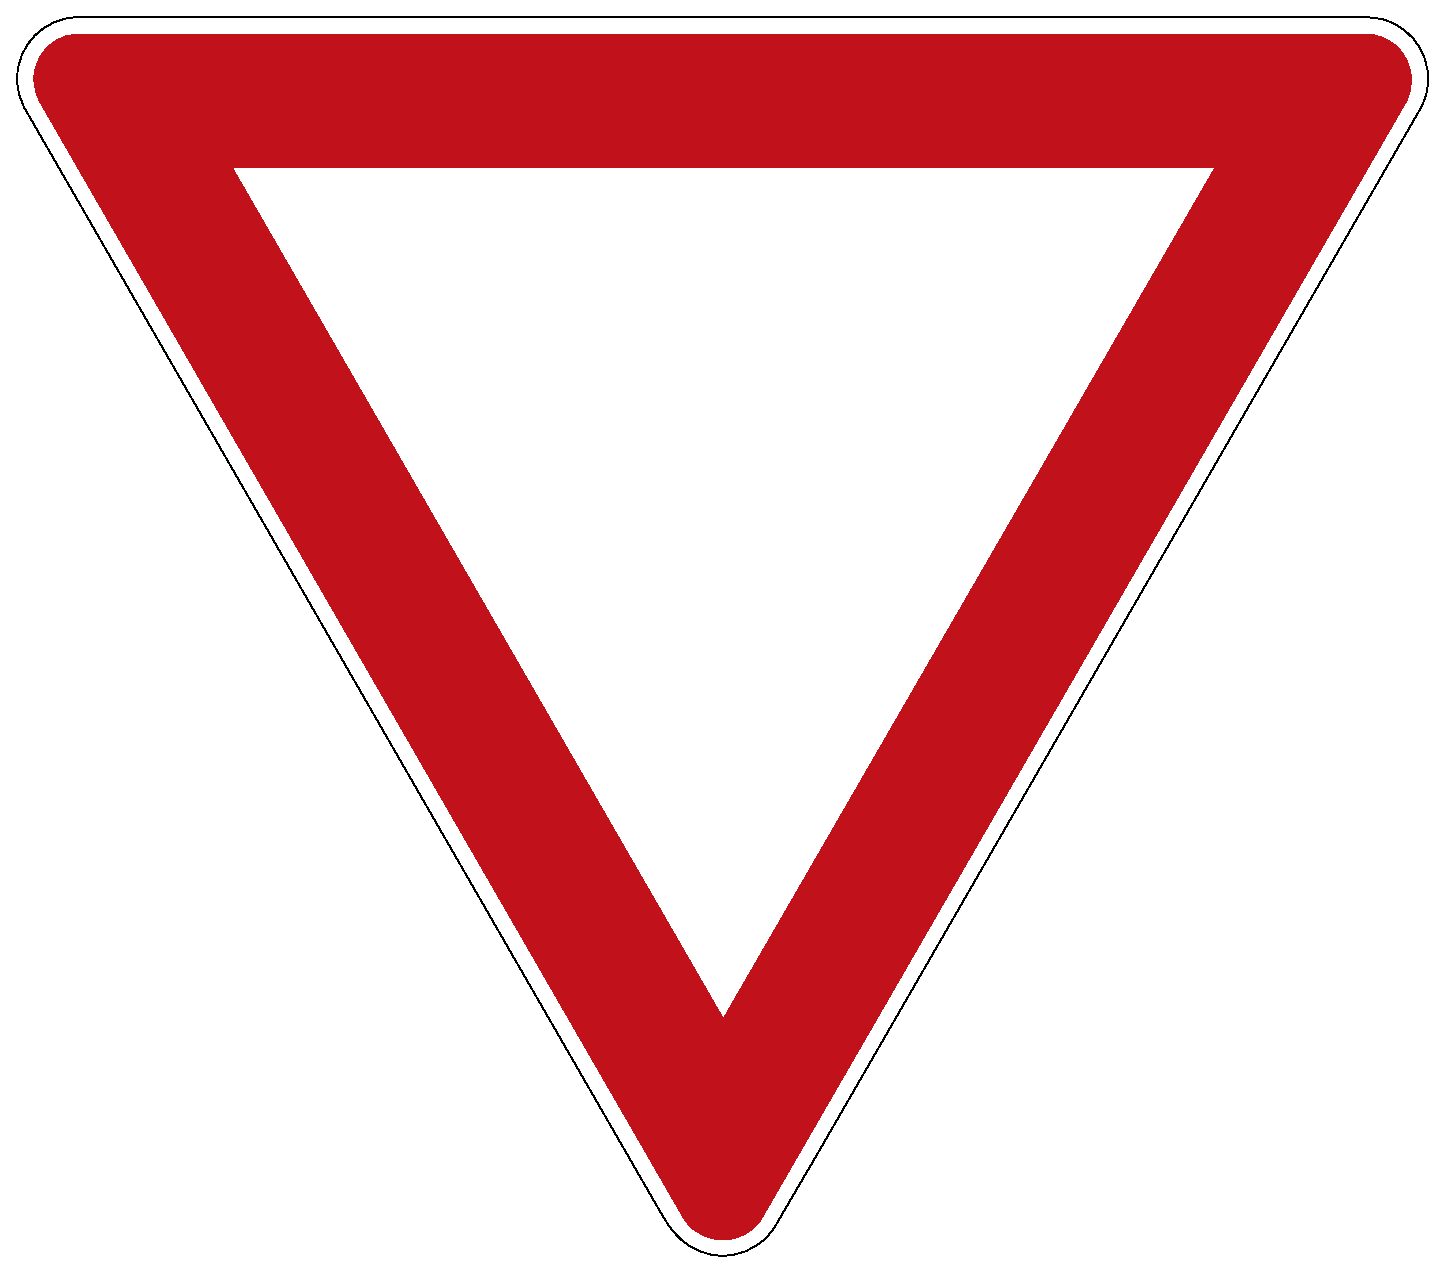
\includegraphics[scale=0.03]{{./figures/205.eps}} & Yield &  205\\
		
\includegraphics[scale=0.04]{{./figures/206.eps}}& Stop & 206\\
		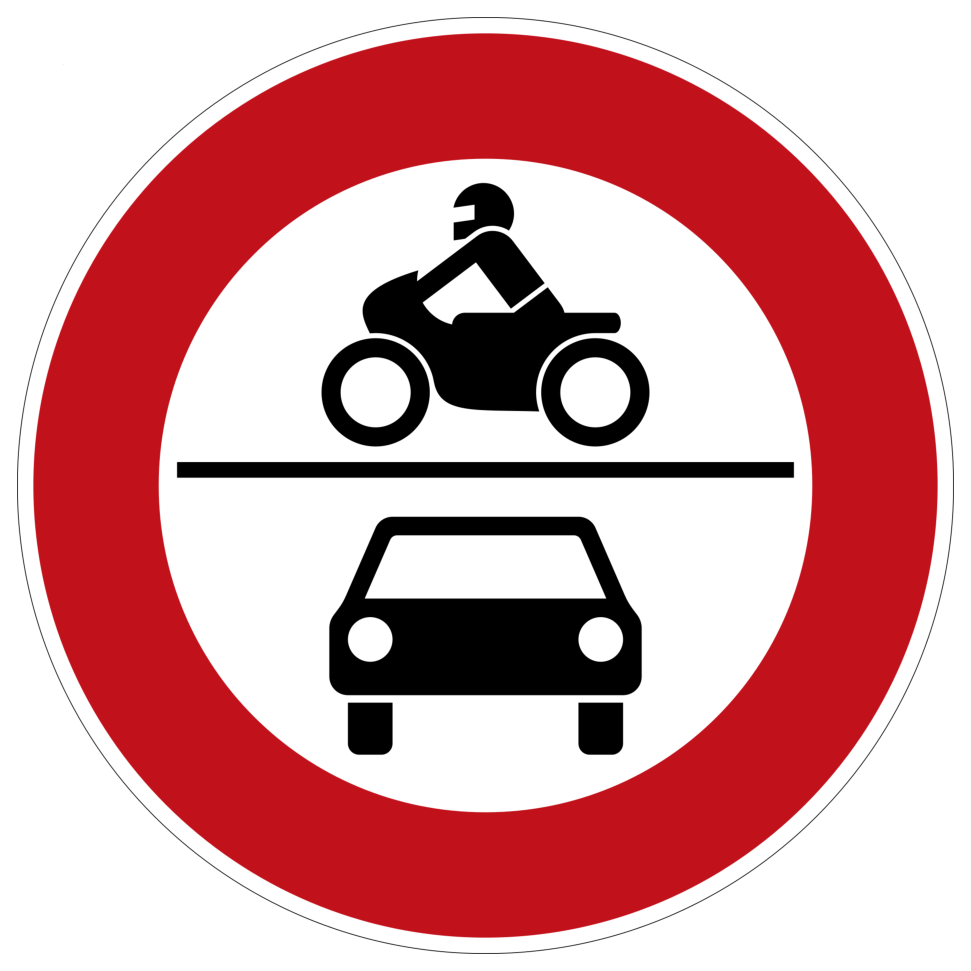
\includegraphics[scale=0.04]{{./figures/260.eps}} & Ban on motorcycles and multi-lane vehicles & 260 \\	
		
\includegraphics[scale=0.04]{{./figures/272.eps}} & No U-turn & 272 \\
		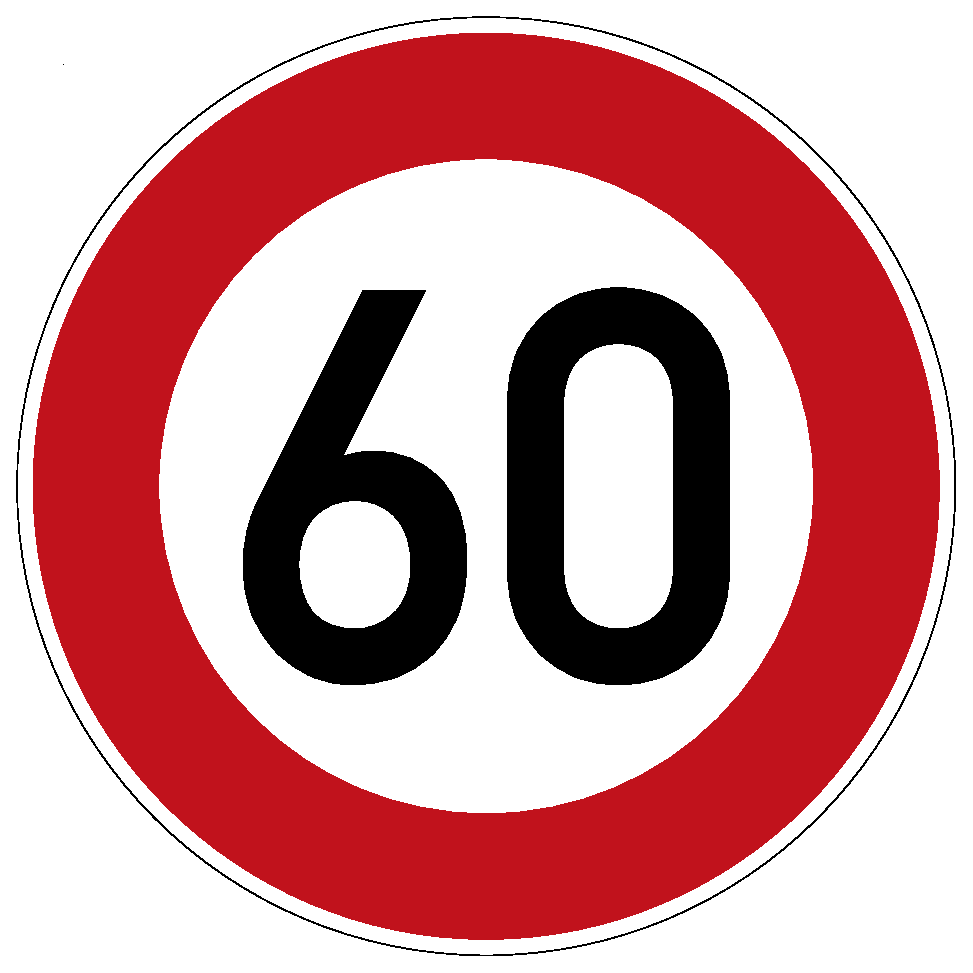
\includegraphics[scale=0.04]{{./figures/274.eps}}& Speed limit & 274 \\
		
\includegraphics[scale=0.04]{{./figures/275.eps}}& Required speed & 275 \\
		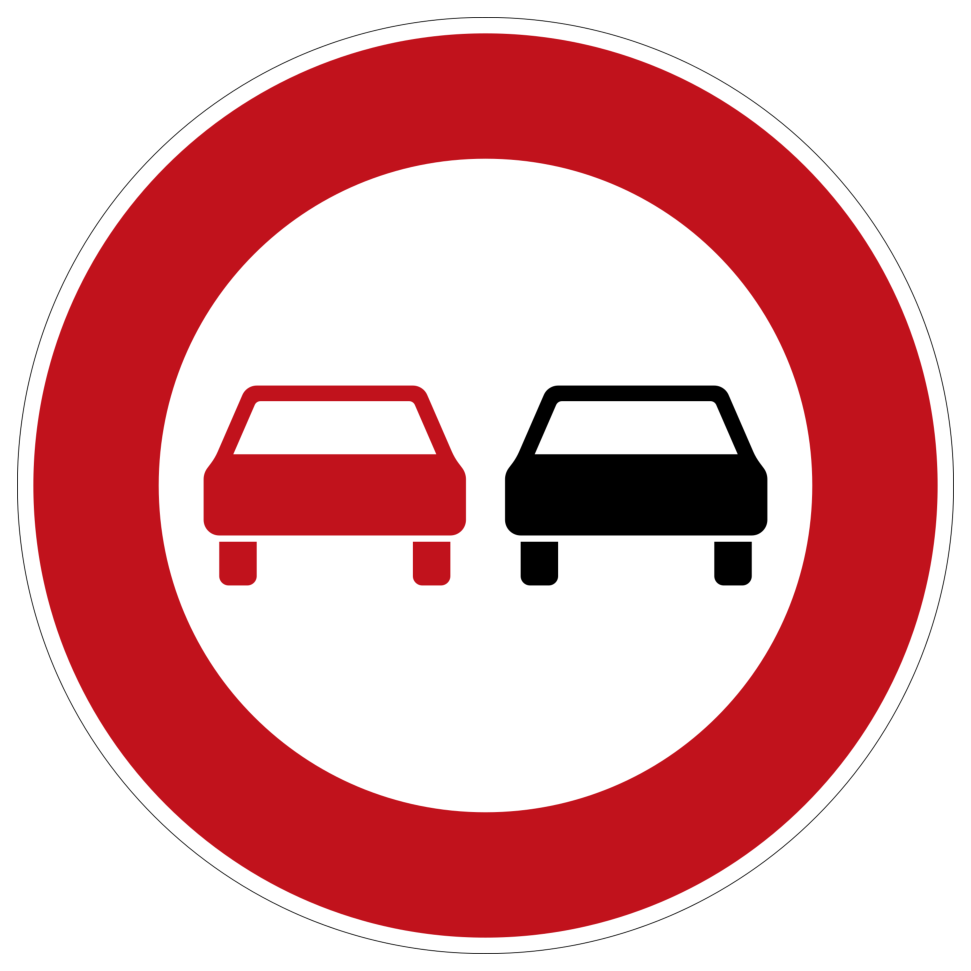
\includegraphics[scale=0.04]{{./figures/276.eps}}& No overtaking (except of non-motorized traffic participants, trains, and motorcycles without sidecar) & 276 \\
		
\includegraphics[scale=0.035]{{./figures/301.eps}} & Right of way & 301\\
		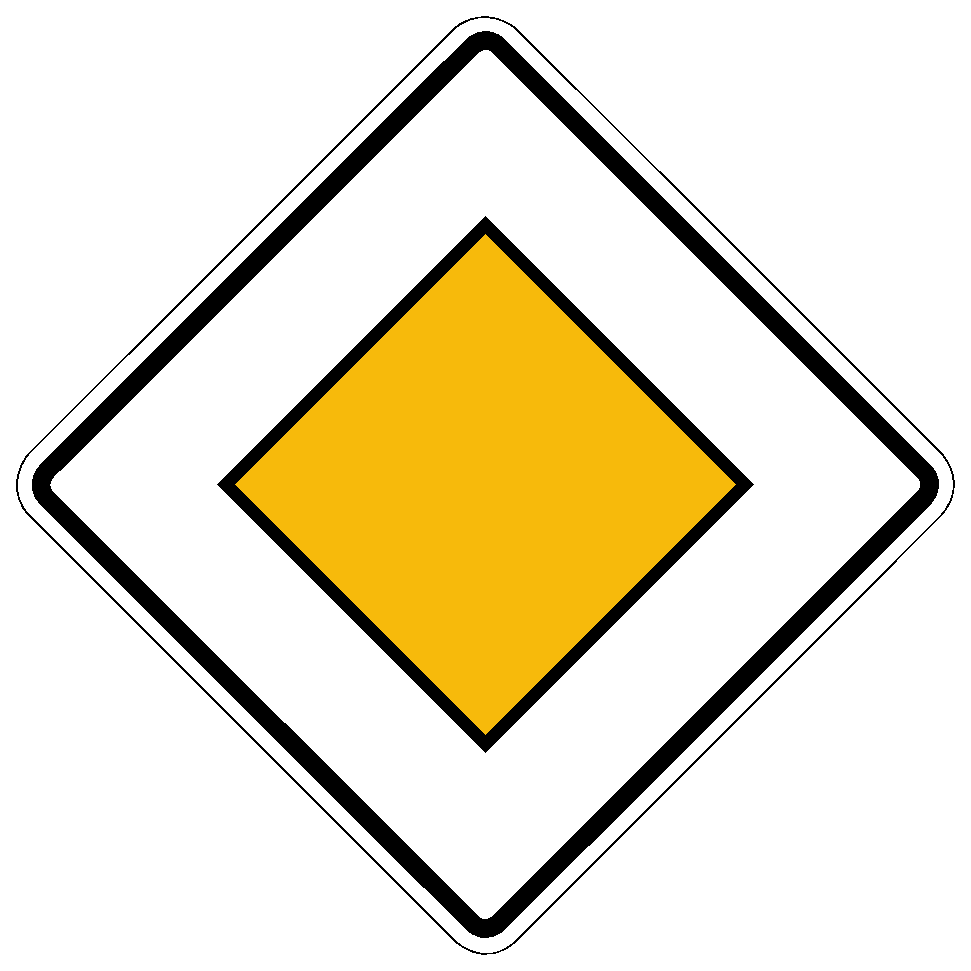
\includegraphics[scale=0.04]{{./figures/306.eps}} & Priority road & 306\\
		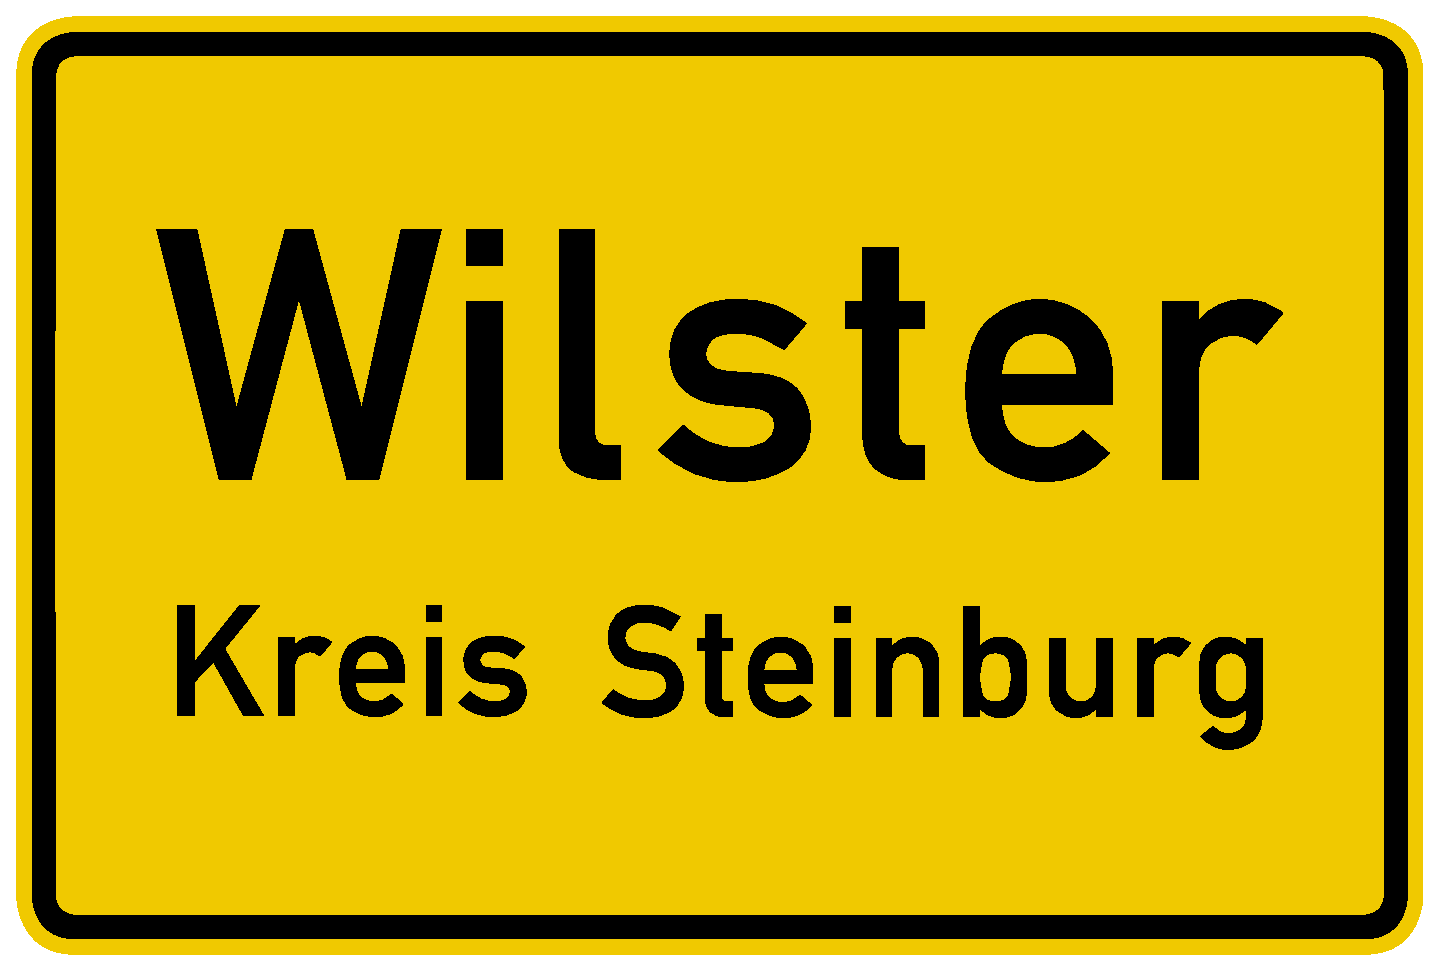
\includegraphics[scale=0.04]{{./figures/310.eps}} & Town sign & 310 \\
		
\includegraphics[scale=0.04]{{./figures/720.eps}} & Green arrow sign & 720 \\
		\bottomrule
	\end{tabular}
	\label{tab:traffic_signs}
\end{table}

\begin{table}[!htb]\centering
	\caption{Overview of all supported traffic signs. Valid for complete lanelet expresses that the traffic sign is always valid from the start of a lanelet. All traffic signs which are not mentioned in this list are valid starting starting from the end of a lanelet.}
	\ra{1.3} 
	\begin{tabular}{@{}lp{9cm}p{4cm}@{}} \toprule
		\textbf{Country} & \textbf{Traffic Sign ID} & \textbf{Valid for complete lanelet} \\ \midrule
		Germany & 101, 102, 108, 114, 123, 138, 142-10,
		201, 205, 206, 208, 209-10, \mbox{209-20}, \mbox{220-10}, \mbox{220-20}, \mbox{222-10}, \mbox{222-20} ,237, 239, 242.1, 242.2, 244.2, 
		244.2, 245, 250, 251, 253, 254, 255, \mbox{257-54}, 259, 260, 261, 262, 264, 265, 266, 26, 272, 
		274, 274.1, 274.2, 275, 276, 277, 278, 281, 282, 301, 306, 308, 310, 325.1, 
		325.2, 327, 330.1, 330.2, 331.1, 331.2, \mbox{333-21}, 333-22, 350, 357, 
		\mbox{625-10}, \mbox{625-11}, \mbox{625-12}, \mbox{625-13}, \mbox{625-20}, \mbox{625-21}, \mbox{625-22}, \mbox{625-23}, \mbox{626-10}, \mbox{626-20}, \mbox{626-30}, \mbox{626-31}, 720, 
		\mbox{1000-10}, \mbox{1000-11}, \mbox{1000-20}, \mbox{1000-21}, \mbox{1000-30}, \mbox{1000-31}, \mbox{1001-30}, \mbox{1001-31}, \mbox{1002-10}, \mbox{1002-12}, \mbox{1002-13}, 
		\mbox{1002-20}, \mbox{1002-22}, \mbox{\mbox{1002-23}, 1002-11}, \mbox{1002-14}, \mbox{1002-21}, \mbox{1002-24}, \mbox{1004-30}, \mbox{1004-31}, \mbox{1020-30}, \mbox{1022-10}, \mbox{1024-10}, \mbox{1026-36}, \mbox{1026-37}, \mbox{1026-38}, \mbox{1040-30}, \mbox{1053-33} & 
		101, 102, 108, 114, 123, 138, 142-10, 201,
		208, 209-10, 209-20, 220-10, 220-20, 222-10, 222-20, 237, 239, 242.1, 244.1, 245, 250, 251, 253, 254, 255, 257-54, 259, 260, 261, 262, 264, 265, 266, 267, 274, 274.1, 275, 276, 277,
		308, 310, 325.1, 327, 330.1, 331.1 \\
		USA & R2-1, R3-4 & R2-1 \\
		\bottomrule
	\end{tabular}
	\label{tab:supportedNationalTrafficSigns}
\end{table}


\subsection{Traffic Lights} \label{subsec:traffic_lights}
The element \textit{trafficLight} is used to represent traffic lights within the scenario (see Fig.~\ref{fig:trafficLight}). Each phase/color of a \textit{trafficLight} and its duration is defined by the element \textit{cycleElement}. Similarly to the \textit{time} elements, the duration is not given as numeric value, but as integer. The color value inactive indicates that currently no phase is activated, e.g. a green right arrow traffic light can be activated iteratively. The order of the different phases is determined by the order of the \textit{cycleElements} in the element \textit{cycle}. By specifying the element \textit{timeOffset}, the cycle is shifted by this value. 

In order to define for which driving direction the traffic light is valid, i.e., the direction arrow(s) in a traffic light, the direction can be included. If the direction is not specified, the traffic light is valid for all directions. Additionally, the element \textit{active} can be used to determine whether a traffic light is active or not. Optionally, the position of the traffic sign can be included. Traffic lights are always valid starting from the end of a lanelet. 

\begin{figure}[!htpb]
	\small
	\dirtree{%
		.1 trafficLight (id).
		.2 [1] cycle.
		.3 [1..N] cycleElement.
		.4 [1] duration.
		.4 [1] color: red/redYellow/green/yellow/inactive.
		.3 [0..1] timeOffset.
		.2 [0..1] position.
		.3 [1] point.
		.2 [0..1] direction: right/straight/left/leftStraight/straightRight/leftRight/all.
		.2 [0..1] active: true/false.
	}
	\caption{Element \textit{trafficLight}.}
	\label{fig:trafficLight}
\end{figure}

%The length of each state of the traffic light is specified by the elements \textit{red}, \textit{redYellow}, \textit{green} and \textit{yellow}.
\newpage
\subsection{Intersections}  \label{subsec:intersections}
The element \textit{intersection} is used to represent an intersection within the road network (see Fig.~\ref{fig:intersection}). An \textit{intersection} element is defined by at least one \textit{incoming}, which consist of \textit{incomingLanelets}, \textit{outgoingsRight}, \textit{outgoingsStraight}, \textit{outgoingsLeft}, the element \textit{isLeftOf}, and the element \textit{crossing}. 

The elements \textit{outgoingsRight}/\textit{Straight}/\textit{Left} are used to infer for which lanelets the traffic light is valid for and to facilitate the calculation of priorities at intersections. The element \textit{isLeftOf} is used to infer the right-before-left-rule. The element \textit{crossing} models lanelets which cross other lanelets, e.g., crosswalks. Since all elements of a \textit{incoming} are already existing, we use an attribute referring to their unique ID. An example for an \textit{intersection} with all elements except crossings is illustrated in Fig.~\ref{fig:intersection}.
\begin{figure}[!htb]
	\centering
	\footnotesize
	\psfrag{A}[l][c]{incoming}	
	\psfrag{B}[l][c]{outgoingsRight}
	\psfrag{C}[l][c]{outgoingsStraight}
	\psfrag{D}[l][c]{outgoingsLeft}
	\psfrag{E}[l][c]{isLeftOf}
	\psfrag{F}[l][c]{crossing}
	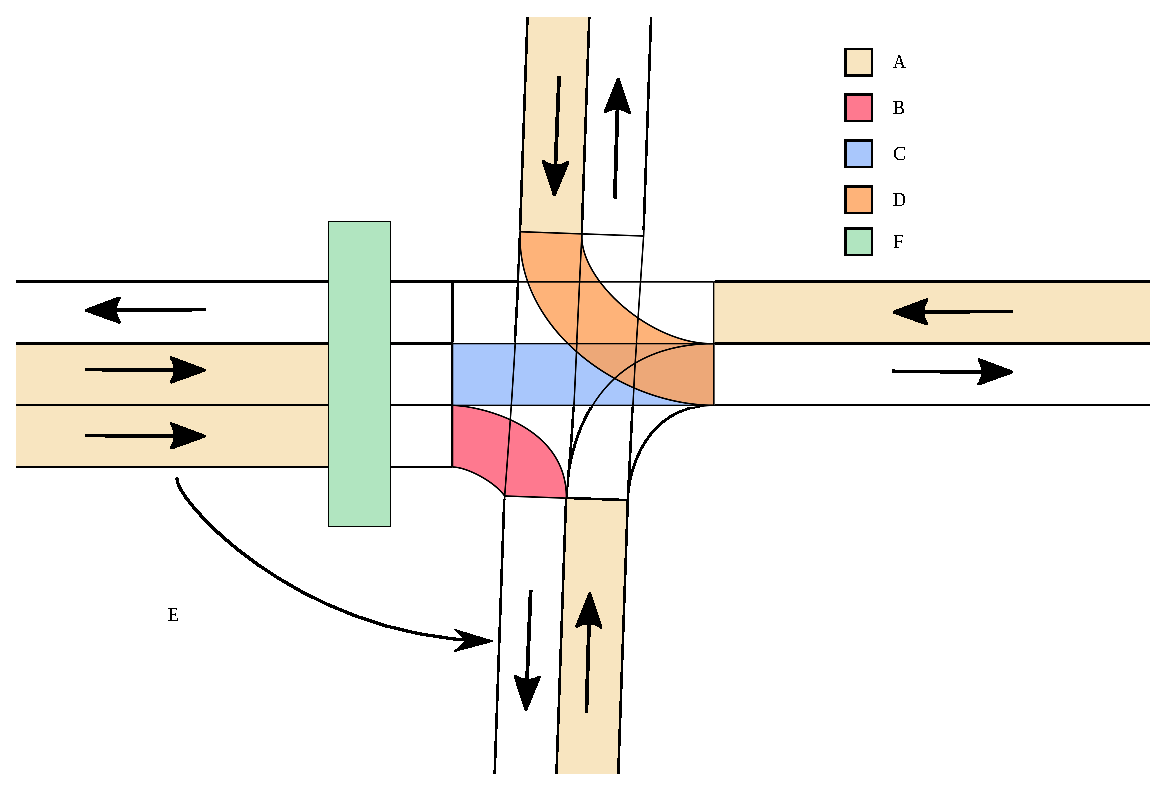
\includegraphics[width=0.6\columnwidth]{figures/intersection.eps}
	\caption{Example intersection. For better visibility, only one example lanelet is highlighted for each outgoingsRight/Straight/Left element.}
	\label{fig:intersection}
\end{figure}
\begin{figure}[!htb]
	\small
	\dirtree{%
		.1 intersection (id).
		.2 [1..N] incoming (id).
		.3 [1..N] incomingLanelet (\textrm{ref to} lanelet).
		%	.4 [0..1] stopLine.
		%	.5 [2] point.
		%	.3 [0..N] trafficSign.
		%	.3 [0..N] trafficLight.
		.3 [0..N] outgoingsRight (\textrm{ref to} all lanelets that complete the right turn within this intersection).
		.3 [0..N] outgoingsStraight (\textrm{ref to} all lanelets that are going straight).
		.3 [0..N] outgoingsLeft (\textrm{ref to} all lanelets that are turning left).
		.3 [0..1] isLeftOf (\textrm{ref to} incoming).
		.2 [0..N] crossing.
		.3 [1..N] crossingLanelet (\textrm{ref to} lanelet (usually of type crosswalk)).
		%	.3 [0..N] trafficSign.
		%	.3 [0..N] trafficLight.
	}
	\caption{Element \textit{intersection}.}
	\label{fig:intersection}
\end{figure}

\footnotetext{\href{https://commons.wikimedia.org}{commons.wikimedia.org}}


\subsubsection{Environment Obstalces}
The element \textit{environmentObstacle} is used to specify the outline of environmental or infrastructure objects to properly compute occlusions. A \textit{environmentObstacle} is specified by its type, e.g. building, and its shape. 

